\documentclass[12pt]{article}

\usepackage{amsmath}
\usepackage{mathtools}
\usepackage{algorithm}

\usepackage{algorithmic}

\usepackage{enumitem}

\usepackage{amssymb}
\usepackage[T1]{fontenc}
\usepackage{float}
\usepackage{graphicx}

\usepackage{hyperref}
\hypersetup{
    colorlinks=true,
    linkcolor=blue,
    filecolor=magenta,      
    urlcolor=cyan,
    bookmarks=true,
}
\usepackage[font=footnotesize]{caption}
\setcounter{secnumdepth}{4}
\usepackage[utf8]{inputenc}
\begin{document}
    Cette version de l'algorithme, proposée dans \cite{abdel2018improved} utilise une fonction à dynamique chaotique et la distribution vol de Lévy afin de garantir une convergence rapide. Une phase de mutation est aussi rajoutée à la fin de chaque itération 
\subsection{Fonction à dynamique chaotique}
Soit f:I $\rightarrow$ I une fonction continue.On suppose que la dynamique associée est chaotique.Alors:
\begin{enumerate}
    \item L'ensemble des points périodiques de f est partout dense dans I 
    \item f est sensible aux conditions initiales, ceci signifie que s'il y'a un petit changement dans la condition initiale $x_0$,le changement correspondant de $x_t=f_t(x_0)$ croit avec la croissance de t 
\end{enumerate}
Ce sont des fonctions qui permettent d'avoir une suite de nombres aléatoires qui dépend d'une condition initiale.Il existe plusieurs types de fonctions chaotique :fonction logistique,fonction de tchebychev.Après plusieurs tests, il a été remarqué qu'avec les fonctions logistiques nous obtenons une convergence plus rapide de la fonction objective .Le minimum de la fonction objective a été atteint en 5 itérations comme le montre le graphe
\begin{figure}[H]
   \centering
    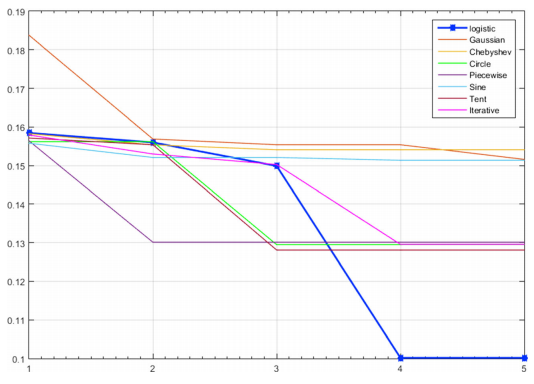
\includegraphics[width=10cm]{../figures/logisticvsothers.PNG}
    \caption{convergence fonctions chaotiques \cite{abdel2018improved}}
\end{figure}
Du graphe , on peut voir qu'avec la fonction logistique la fonction objective atteint le minimumu à partir de la 5eme itération
\subsubsection{Fonction logistique}
La fonction logistique est définie par la formule suivante :
\newline
\begin{center}
    $x_{n+1}=ax_n(1-x_n) ,x\in[0,1],0<a\leq4$   
\end{center}
où a est une constante caractéristique de la fonction logistique que nous avons fixé à la valeur give the value après plusieurs simulations
La fonction logistique est utilisée dans l'algorithme pour générer la valeur p
\subsection{La distribution vol de Lévy}
le vol de levy est un modèle mathématique caractérisé par une moyenne et une variance infinies ce qui rend le mouvement plus lent permettant ainsi une meilleure exploration de l'espace de recherche \cite{JAMIL201349}.
Dans ILWOA , la variable C est remplacé par un pas aléatoire de la marche aleatoire levy donné par les formules suivantes:
\begin{align*}
&Levy\leadsto\frac{\lambda\Gamma(\lambda)\sin(\pi\lambda/2)}{\pi}\frac{1}{s^{1+\lambda}}\\
&s=\frac{U}{\left|{V^{\lambda^-1}}\right| },\quad U\leadsto N(0,\sigma_u^2),V\leadsto N(0,1)\\
&\sigma_u^2=[\frac{\Gamma(\lambda+1)}{\Gamma((\lambda+1)/2)}\frac{\sin(\pi\lambda/2)}{2^{(\lambda-1)/2}}]^{1/\lambda}
\end{align*}
\subsection{Phase de mutation}
Une phase de mutation a lieu à la fin de chaque itération. On vérifie d'abord si la solution atteinte est optimale .dans ce cas la recherche s'arrete sinon on applique la mutation sur cette dernière.
Cette phase est composée de 3 opérations exécutées séquentiellement comme le montre la figure \textbf{\emph{\refeq{fig:mutation}}}: 
\begin{itemize}
    \item Permutation: deux items de la solution sont choisis aléatoirement pour effectuer une permutation entre eux
    \item Deplacement: Un sous ensemble d'items choisi aléatoirement est déplacé vers une position qui est egalement choisie aléatoirement
    \item Inversion: On applique une inversion sur un sous ensemble d'items
\end{itemize}
\begin{figure}[h!]
   \centering
    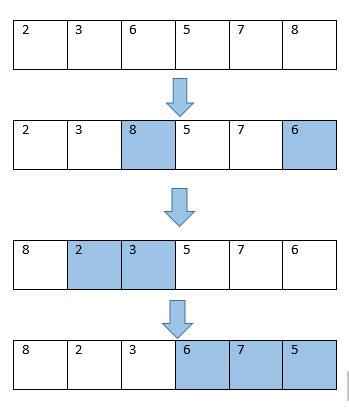
\includegraphics[width=10cm]{../figures/Mutation.PNG}
    \caption{Phase de mutation}
    \label{fig:mutation}
\end{figure}
\subsection{Pseudocode}
\begin{algorithm}[H]
    \caption{Improved Whale Optimization Algorithm}
    \begin{algorithmic}
        \STATE Initialiser la population de baleines (l'ensemble initial des solutions candidates): Xi (i = 1, 2 ,..., N)\;
        \STATE Évaluer les solutions de la population initiale\;
        \STATE X* = la meilleure solution actuelle\;
        \WHILE{\(t < max\_iter\)}
            \FOR{solution \(\in\) population}
                \STATE Mettre à jour a, A, C avec le vol de levy, l et p avec la fonction logistique\;
                \IF{\(r  < 0,5\)}
                    \IF{\(|A| < 1\)}
                        \STATE Mettre à jour la solution par Eq.(1)\;
                    \ELSE
                        \STATE Sélectionner une solution aléatoire \(X_r\)\;
                        \STATE Mettre à jour la solution par Eq.(2)\;
                    \ENDIF
                \ELSE 
                    \STATE Mettre à jour la solution par l'Eq.(3)\;
                \ENDIF
            \ENDFOR
            \STATE Vérifier si une solution dans la population dépasse l'espace de recherche et la modifier\;
            \STATE Appliquer la discretisation par LOV\;
            \STATE Évaluer la nouvelle solution\;
            \STATE Mettre à jour X* s'il existe une meilleure solution Sinon lancer la phase de mutation\;
            \STATE Evaluer la nouvelle solution,màj de la meilleure solution
            \STATE t = t + 1\;
        \ENDWHILE
    \end{algorithmic}
\end{algorithm}
\subsection{Test et résultats}
Pour montrer les performances de cet algorithme nous avons effectué une série de Test sur des instances du Benchmark \guillemotleft Scholl \guillemotright composé de trois classes d’une difficulté qui varie d’une classe à une autre.
En ce qui concerne les paramètres de l’algorithme, nous avons utilisé deux méthodes de calibrage : Un calibrage manuel et un calibrage automatique avec IRace; Le tableau dans la \textbf{\emph{figure \refeq{tab:table1}}} indique les valeurs obtenues par chacune des deux méthodes.
\begin{table}[h!]
    \begin{center}
      \caption{Configuration paramétrique de l'algorithme}
      \label{tab:table1}
      \begin{tabular}{c|c|c|c|c|c} % <-- Alignments: 1st column left, 2nd middle and 3rd right, with vertical lines in between
       \textbf{}&\textbf{a} & \textbf{b} &\textbf{beta} & \textbf{max\_iter} & \textbf{nb\_whales} \\
        \hline
        
        Calibrage manuel &8&0.99&1.5&391&13\\ 
        \hline
       Calibrage automatique&4&1.5&1&30(Hard),10(Classe 1 et 2)&10\\
        \hline
      \end{tabular}
    \end{center}
  \end{table}
\linebreak
 Nous allons dans l’analyse qui suit:
\begin{itemize}
    \item comparer entre les résultats obtenus par les deux méthodes de calibrage ainsi montrer l’influence du choix des paramètres sur la performance de l’algorithme.
    \item Analyser les performances de l’algorithme et le comparer à l’algorithme WOA exécuté avec la configuration optimale suivante : $nb\_whales=28$, $max\_iter=271$,  $b=7.64$, $a=20$ .
\end{itemize}
\subsubsection{Comparaison entre les résultats obtenus par calibrage automatique et les résultats obtenus par calibrage manuel:                }
Afin d’effectuer cela, nous avons exécuté l’algorithme avec les paramètres obtenus par calibrage automatique et les paramètres obtenus par calibrage automatique, sur les instances difficiles de la classe 3. Les tableaux dans la \textbf{\emph{figure \refeq{tab:calib_c3}}} montrent que le calibrage automatique améliore la qualité de la solution ainsi que le temps d’exécution
\begin{figure}[h!]
    \centering
     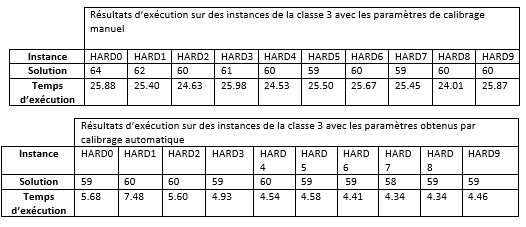
\includegraphics[width=10cm]{../figures/tabreslts.PNG}
     \caption{Résultats d'exécution des instances de la classe 3 avec calibrage manuel vs. calibrage automatique.}
     \label{tab:calib_c3}
 \end{figure}
\subsubsection{Analyse des performances de l'algorithme: }
\paragraph{Analyse du temps d'exécution:}
A partir du graphes \textbf{\emph{figure \refeq{fig:texec_comp}}} , on peut déduire que :
\begin{itemize}
    \item Le temps d'exécution de ILWOA varie de 1  à quelques dizaines de secondes pour les grandes instances 
    \item L’algorithme ILWOA est plus lent que WOA , on justifie ceci par le fait qu’en plus des instructions exécutées par le WOA , l’ILWOA comporte une phase de mutation et une initialisation par une heuristique  
\end{itemize}
\begin{figure}[h!]
    \centering
     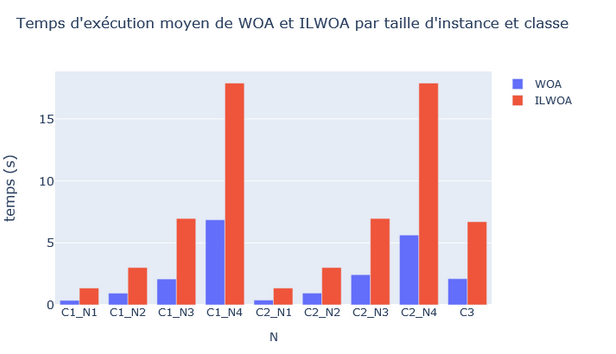
\includegraphics[width=10cm]{../figures/woavsilwoatemps.PNG}
     \caption{temps d'execution (en s) de ILWOA et WOA}
    \label{fig:texec_comp}
    \end{figure}
 \paragraph{Analyse de la qualité de solution: }La qualité de solution a été mesurée par le ration dont on a cité la formule précédemment.A partir du graphes ci-dessous , on peut déduire que :
 \begin{itemize}
     \item Le Ratio obtenu par l’ILWOA est proche de 1 pour toutes les instances même pour les instance de la classe 3 ceci signifie qu’il donne de bons résultats quelque soit la difficulté de l’instance 
     \item la solution obtenue avec l’algorithme ILWOA est très proche de la solution optimale voire même égale pour des instances des classes 1 et 2 
     \item ILWOA améliore la qualité de solution par rapport à l’algorithme woa pour les instances des 3 classes confondues
 \end{itemize}
 \begin{figure}[h!]
     \centering
      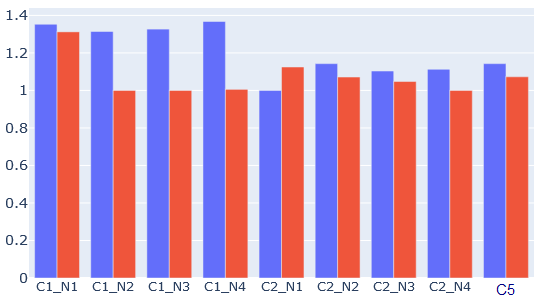
\includegraphics[width=10cm]{../figures/ratio_ilwoa_woa}
      \caption{ratio de ILWOA et WOA}
  \end{figure}
  \subsubsection{Interprétation }
  \begin{itemize}
    \item L’Algorithme ILWOA permet d’obtenir une bonne qualité de solution en un temps raisonnable   
    \item Le caractère stochastique de l’algorithme WOA permet de mieux explorer l’espace de recherche, l’utilisation des fonctions logistiques et de la distribution du vol de lévy ont amélioré cela 
    \item En analysant le nombre de search agents et d’itérations ainsi que la solution obtenue , On peut conclure que l’ajout d’une phase de mutation a permis d’améliorer la rapidité de convergence de l’algorithme 
    \item Les améliorations effectuées ont permis d’augmenter la performance de l’algorithme 
    \item La performance de l’algorithme dépend fortement des valeurs de ses paramètres d’où la nécessité du calibrage qui permet de trouver la meilleure configuration pour l’algorithme
    \item La valeur des paramètres peut dépendre de la nature de l’instance
    \item Le calibrage automatique est important du fait que ça permet de nous épargner une tâche tant  fastidieuse, tout en assurant une meilleure qualité du résultat

\end{itemize}


\end{document}